\documentclass{article}
\usepackage[utf8]{inputenc}
\usepackage[T1]{fontenc}
\usepackage{graphicx}
\usepackage{amsmath}
\usepackage{wrapfig}
\usepackage[top=1in, bottom=1.25in, left=1.1in, right=1.1in]{geometry}

\title{Reporte - Actividad 3: Sondeos Meteorológicos}
\author{García Monge Itzel Alexia}
\date{15 de Febrero, 2018}

\begin{document}
\maketitle
\section{Introducción}
El siguiente reporte muestra el procedimiento y resultados de la práctica tres de física computacional, en donde se le dió seguimiento a la programación con Python, aprendiendo a seleccionar qué leer y qué ignorar de una tabla de datos proporcionada por los sondeos atmosféricos de la Universidad de Wyoming, así como cambiar el tipo en el que se leen los datos para finalmente graficarlos.

\section{Fundamentos}
Antes de lograr iniciar con la explicación de la actividad, se debe de tener bien entendido lo que son los sondeos meteorológicos. Las sondas comúnmente utilizadas para los sondeos meteorológicos son una pequeña caja electrónica de plástico no muy pesada con sensores, procesador de señales, transmisor de radio y baterías. Para que las sondas logren obtener los valores de las capas atmosféricas se cuelgan de un hilo de 30 $m$ de largo a un globo de goma natural, llenándolos hasta 1.2 $m$ de su diámetro inicial comúnmente con hidrógeno  helio, haciendo que el globo se eleve hacia la atmósfera. El conjunto de la sonda amarrada al globo se denomina globo sonda.

	Durante el ascenso se logra medir la temperatura ambiente, el punto de rocío, la presión, la velocidad y dirección del viento utilizando posicionamiento en tres dimensiones mediante el uso de los GPS. La sonda no sube estrictamente de manera vertical a causa del viento, pero al ser los gradientes horizontales de
las magnitudes atmosféricas mucho menores que los verticales, no afecta sus mediciones, las cuales tampoco están sincronizadas.

	El sensor de temperatura suele ser un termistor de baja inercia con recubrimiento reflectante y de baja emisividad para minimizar el intercambio radiativo, calibrado para dar una precisión de $\pm$ 0.1 $^\circ$C en el rango -90 a 50 $^\circ$C. El sensor de humedad, el cual tiene una capa que lo protege de las precipitaciones, suele ser una delgada lámina dieléctrica entre electrodos, formando un condensador cuya capacidad eléctrica varía con la humedad relativa del aire ambiente con una respuesta rápida y una precisión mejor del 5\% en todo el rango. El sensor de presión es una cápsula aneroide con transductor capacitivo para la deflexión de la membrana, que ha de ser de alta precisión.
    
    Mediante se sigue ascendiendo, la presión exterior del globo disminuye exponencialmente, haciendo que la goma se vaya expandiendo por sobrepresión. Cuando el globo llega a una altitud aproximada de 30 $km$ hasta que alcanza los 30 km de altitud y se produce su rotura natural. La sonda cuenta con paracaídas, el cual es colocado en el hilo del globo, ayudando a que esta descienda lentamente hacia la tierra nuevamente. Sin embargo, de todas las sondas, sólo se recupera un 20\% o 30\% de ellas.

	Los globos sonda vienen usándose de manera rutinaria desde 1958 para medir perfiles verticales
meteorológicos con detalle que los satélites no son capaces de resolver. Se sueltan varias veces al día en todo el planeta de manera coordinada, utilizando la hora internacional (UTC), desde casi unas mil estaciones meteorológicas a lo largo del planeta. La hora internacional está en relación con la hora solar en el Meridiano de Greenwich.

\section{Análisis de Datos}
Para realizar la actividad se necesitaron de dos tablas, una el 22 de Diciembre y otra el 22 de Junio de la estación Abha en el medio Oriente. Se guardaron los datos de cada estación en las variables $Dec0$ y $Jun0$ ya que se querían utilizar sus datos para realizar gráficas de las temperaturas, vientos y presiones que se experimentaban durante esos dos meses, así que al leer los datos se seleccionó saltarse los primeros 8 o 9 renglones del archivo para que empezara a leer sólo los números. Al hacer eso, se tuvo que volver a nombrar las columnas, lo cual se realizó con la función
	\begin{verbatim}Dec0=pd.read_csv('AbhaDecember.txt', skiprows=8, sep='\s+')
	Jun0=pd.read_csv('AbhaJune.txt', skiprows=9, sep='\s+')
	Dec0.columns=['PRES','HGHT','TEMP','DWPT','RELH','MIXR','DRCT','SKNT','THTA','THTE','THTV']
	Jun0.columns=['PRES','HGHT','TEMP','DWPT','RELH','MIXR','DRCT','SKNT','THTA','THTE','THTV']
    \end{verbatim}

     No todo el documento es la tabla de datos que queremos usar, así que se busca ignorar la información que hay debajo de las tablas. $Drop$ sirve para saltarse cierto número de filas antes de empezar a leer el documento sin eliminarlas. Cuando se quiere saltarse un número de líneas después de haber leído el documento, se utilizan los corchetes, seguido de dos puntos y el número de líneas que se desea eliminar. En este caso se deseaban leer las últimas 21 líneas del Documento Dec0 y las últimas 25 de Jun0.
     
    \begin{verbatim}
    Dec0=Dec0[:-21]
    Jun0=Jun0[:-25]
	\end{verbatim}
    
    El resultado es una tabla donde únicamente aparezcan los datos númericos de cada columna, por ejemplo, el inicio de la tabla de Diciembre es como sigue
    
    \begin{center}
    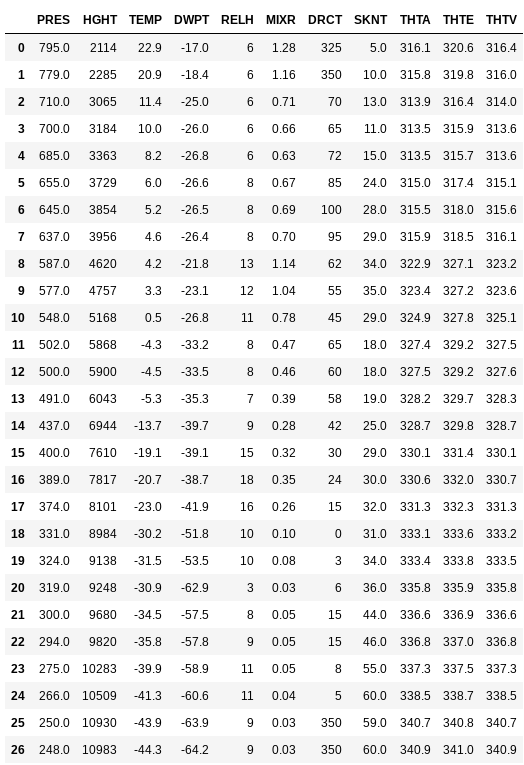
\includegraphics[height=9cm]{TablaDec.png}
    \end{center}
    
    Ya que se tienen los datos necesarios en una tabla, se procede a observar que su $.dtype$ se encuentra en forma de $object$, es decir, en forma de objetos, como palabras. 
    
    \begin{center}
    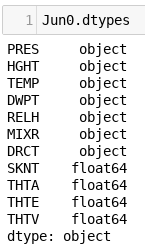
\includegraphics[height=5cm]{JunTypeObj.png}
    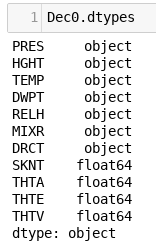
\includegraphics[height=5cm]{dectypeobj.png}
    \end{center}
    
    Para poder graficar los datos se necesitan leer en forma de punto flotante $float64$, entonces se deben de convertir de un tipo a otro, eso es posible utilizando la función

	\begin{verbatim}ConjuntoCol=['PRES','HGHT','TEMP','DWPT','RELH','MIXR','DRCT','SKNT','THTA','THTE','THTV']
	Dec0[ConjuntoCol]=Dec0[ConjuntoCol].apply(pd.to_numeric,errors='coerce',axis=1)
    \end{verbatim}
    
    Entonces al usar la función $.dtype$ esta vez los datos son leídos como punto flotante y al momento de graficar se podrán leer como números.
    
    \begin{center}
    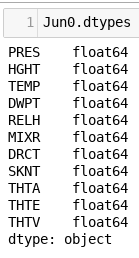
\includegraphics[height=5cm]{JunTypeFlot.png}
    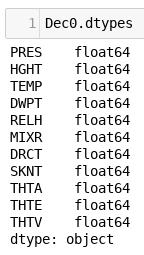
\includegraphics[height=5cm]{DecTypeFlot.png}
    \end{center}
    
    El último procedimiento necesario antes de inicar a graficar que queda es darle estructura a los datos con $pandas$ utilizando $DataFrame$.
    \begin{verbatim}
    Dec=pd.DataFrame(Dec0)
    Jun=pd.DataFrame(Jun0)
    \end{verbatim}
    
    Con los datos seleccionados, del tipo correcto y con estructura, se puede inciar a graficar. Durante esta práctica la mayoría de las graficas se utilizaron como función de la altura. La primera siendo con respecto a la presión, en donde se puede apreciar una función exponencial.
    
    \begin{center}
    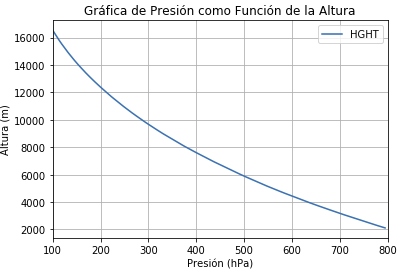
\includegraphics[height=5cm]{PresionDec.png}{Diciembre}
    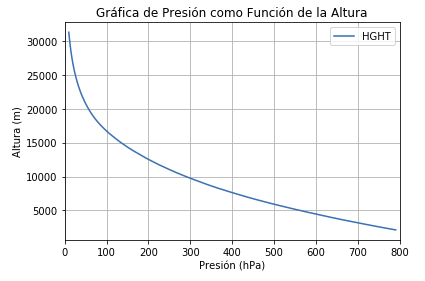
\includegraphics[height=5cm]{PresionJun.png}{Junio}
    \end{center}
    
    Las segundas fueron las temperaturas en función de la altura. Los datos en el sondeo del 22 de Diciembre no alcanzaron una altitud tan alta como el 22 de Junio, pero presentas comportamientos similares en donde se aprecian ambas altitudes.
    
    \begin{center}
    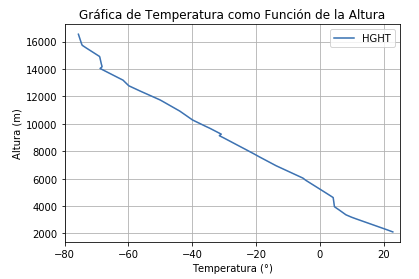
\includegraphics[height=5cm]{TempDec.png}{Diciembre}
    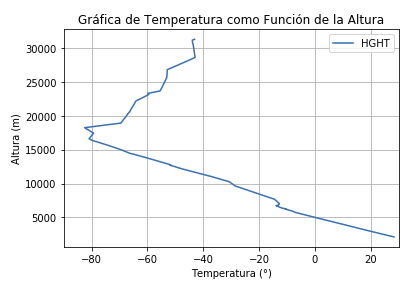
\includegraphics[height=5cm]{TempJun.png}{Junio}
    \end{center}
    
    La tercera era una gráfica de la temperatura y temperatura de rocío, como función de la altura. Durante Diciembre sus comportamientos son constantes, una se mantiene encima de la otra y actúan similarmente a una recta. Durante Junio hay momentos en los que una temperatura se encuentra encima de la otra y no se comportan de manera proporcionada.
    
    \begin{center}
    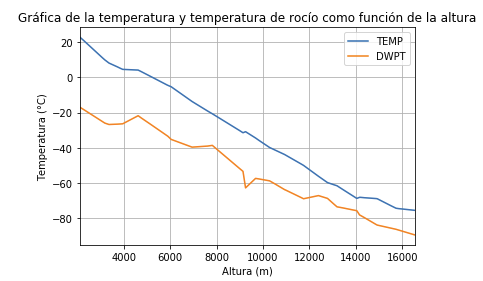
\includegraphics[height=5cm]{DobleDec1.png}{Diciembre}
    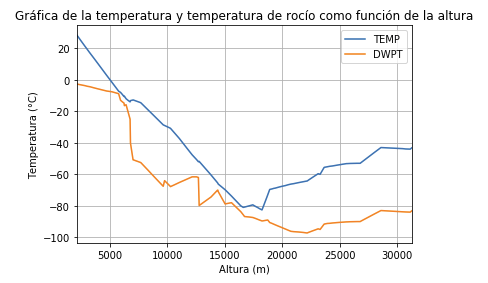
\includegraphics[height=5cm]{DobleJun1.png}{Junio}
    \end{center}
    
    La cuarta fue simplemente una gráfica de la rapidez de los vientos. 
    
    \begin{center}
    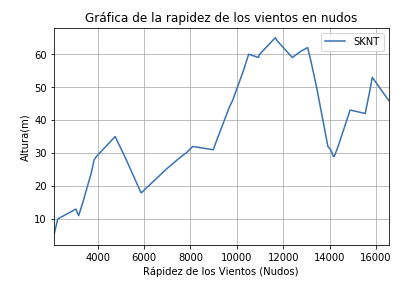
\includegraphics[height=5cm]{VienDec.png}{Diciembre}
    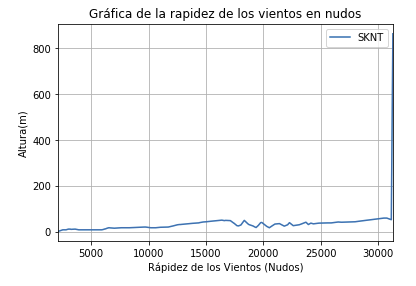
\includegraphics[height=5cm]{VienJun.png}{Junio}
    \end{center}
    
    Mientras que las últimas fueron las gráficas de la humedad relativa en función de la altura. Éstas actuaron en forma esporádica, presentando saltos de humedad drásticos en diferentes altitudes.
    
    \begin{center}
    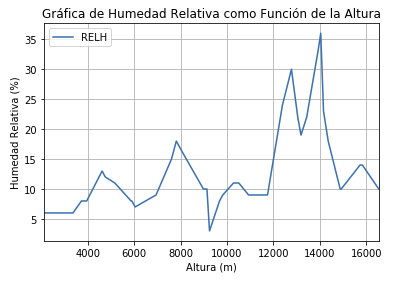
\includegraphics[height=5cm]{HumRelDec.png}{Diciembre}
    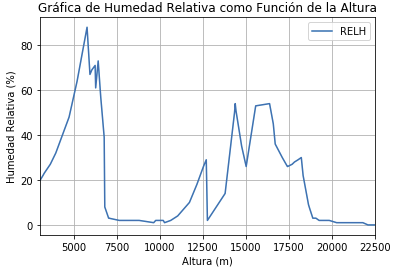
\includegraphics[height=5cm]{HumRelJun.png}{Junio}
    \end{center}
    
\section{Resultados}
En las primeras gráficas, donde se graficó la presión como función de la altura, se observa que sin importar que mes del año sea, la presión disminuye exponencialmente conforme la altura va en aumento. 

	En las segundas gráficas, donde se graficó la temperatura como función de la altura, tampoco se observa un cambio muy notorio entre la gráfica de Junio y Diciembre. Mientras que en Diciembre la altura máxima graficada fue de 16,000 $m$, la altura máxima graficada en Junio fue de 30,000 $m$. Esto hace parecer como si sus gráficas mostraran resultados distintos al de la otra, pero si se comparan ambas hasta los 16,000 $m$, reflejan casi lo mismo.
	
    En la gráfica de temperatura y temperatura de rocío, se puede observar que en Junio es más propensa la temperatura a formar nubes a cierta altura, ya que entre la temperatura de rocio y la temperatura tienen muy poca distancia entre sí, lo que indica que se concentran más las nubes. En cambio, el dia 22 de Diciembre muestra una distancia constante entre la temperatura de rocio y la temperatura, haciendo más difícil que se formen las nubes.
    
    Para la gráficas donde se obtuvo la rápidez de los vientos en nudos se observa que en Diciembre se observan unos vientos tranquilos los cuales aumentan de rapidez conforme se aumentan los valores, mientras que en Junio se experimentan vientos más fuertes.
    
    En las últimas gráficas, las cuales fueron de humedad relativa como función de la altura, se encuentra que en Junio la humedad relativa aumenta drásticamente, formando un pico, entre más se acerca al final de la tropósfera. Mientras que en Junio, la humedad relativa es mucho mayor estando más cerca de la superficie Terrestre.

\section{Conclusión}
La actividad ayudó a crear conciencia sobre la importancia del manejo de datos. Aunque se cuente con una herramienta que facilite la graficación de ellos, los datos son delicados y deben de estar bien estructurados, con el tipo correcto, sin mencionar que sólo se deben de utilizar los datos que vamos a manejar, aprendiendo a descartar cuáles no son necesarios. En general, se aprendió que el manejo correcto de los datos para graficar es lo que toma la mayoría del tiempo y esfuerzo que la graficación en sí.

	%profe, ya me canse aqui se la dejo. me doy de baja lmao bye
	
\section{Bibliografía}
\begin{itemize}
\item Martínez Isidro. (2018). Termodinámica de la Atmósfera. P. 47-48. From

$http://webserver.dmt.upm.es/\sim isidoro/Env/Atmospheric\%20thermodynamics.pdf$
\end{itemize}

\section{Apéndice}
\begin{enumerate}
\item \textbf{¿Cuál es tu opinión general de esta actividad?}
Fue interesante ver que graficar es la parte más rápida y sencilla cuando quieres graficar con muchos datos. Lo que es realmente un trabajo, y no me esperaba que lo fuera, era el "limpiar" los datos, dándoles estructura y convirtiéndolos al tipo correcto.
\item \textbf{¿Qué fue lo que más te agradó? ¿Lo que menos te agradó?} Me agradó el poder experimentar diferentes formas de resolver cómo hacer para no leer partes de un documento, pero no me agradó el hecho que el tipo que leyó los datos brindados fueran de objeto, no importaba qué hiciera, los leía así, y convertirlo a punto flotante fue difícil.
\item \textbf{¿Que consideras que aprendiste en esta actividad?} Cómo limpiar datos para poder graficarlos o interpretarlos sin problema, al menos una forma básica de lograrlo, como cambiar el $.dftype$, darle estructura a la tabla, asignar títulos a las columnas y saltar líneas que no querámos leer.
\item \textbf{¿Qué le faltó? ¿O le sobró?} Faltó un poco más de comprensión sobre el por qué los datos eran leídos como un tipo, aunque se encontró una manera de convertirlo, siento que sería mucho mejor saber por qué ocurre y cómo evitar que vuelva a pasar.
\item \textbf{¿Qué mejoras sugieres a la actividad?} La verdad me pareció una buena práctica, tal vez un poco más de información sobre el maneja de los $.dftypes$, pero en sí la sentí completa.
\end{enumerate}

\end{document}
